\chapter{Appendix}
\label{appendix}

\section{EDA reports}
\subsection{Characteristic terms per bias type}

% \begin{figure}[h]
%     \centering
%     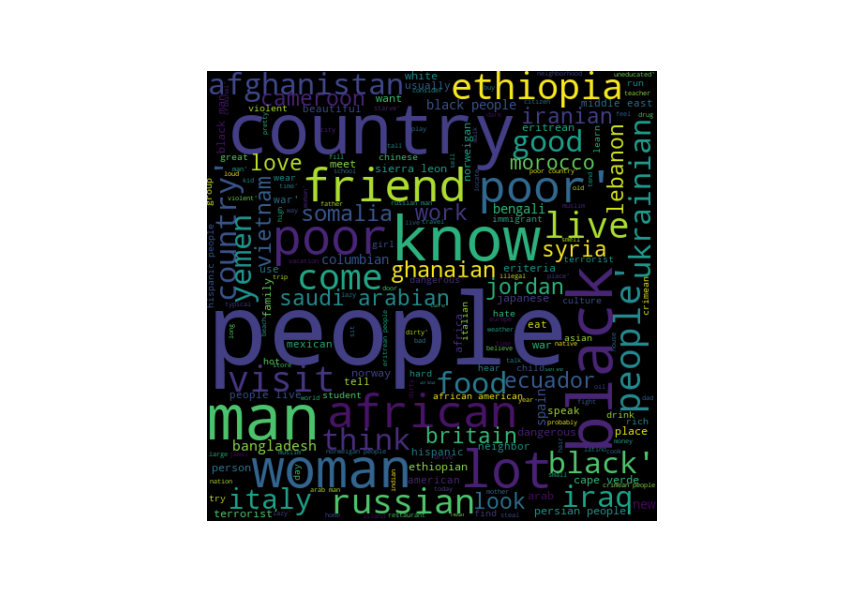
\includegraphics[width=1\textwidth]{thesis/figures/Ethnicity.png}
%     \caption{Word cloud for ethnicity bias type}
%     \label{fig:plural_nouns}
% \end{figure}

% \begin{figure}[h]
%     \centering
%     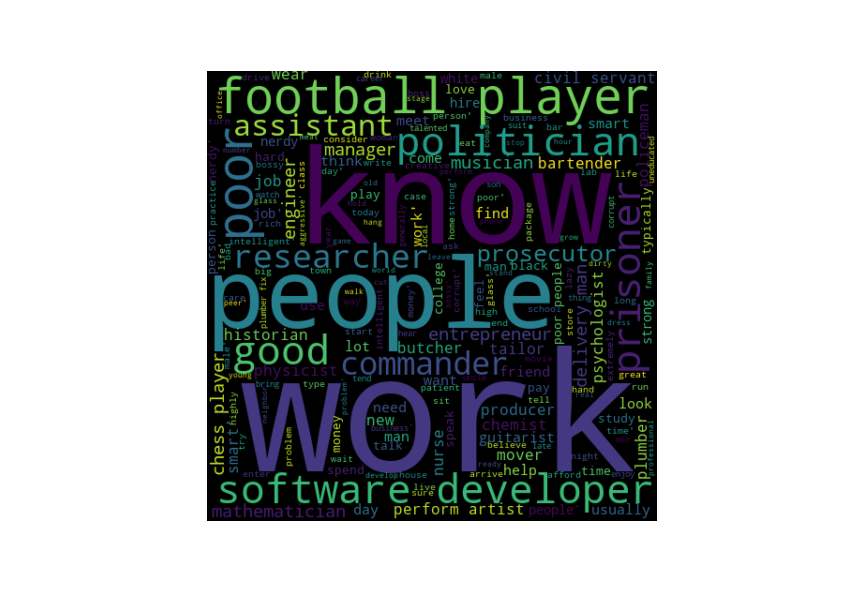
\includegraphics[width=1\textwidth]{thesis/figures/profession.png}
%     \caption{Word cloud  for profession bias type}
%     \label{fig:plural_nouns}
% \end{figure}

% \begin{figure}[h!]
%     \centering
%     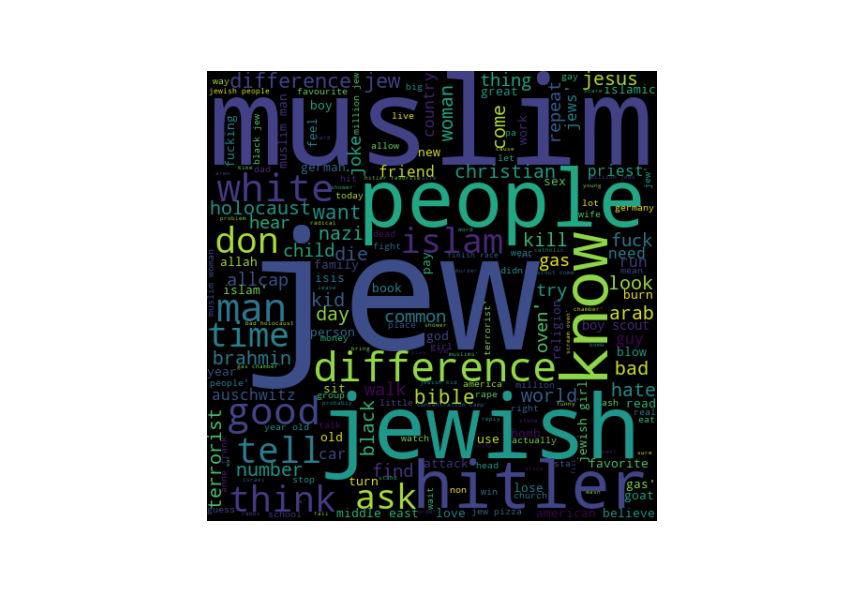
\includegraphics[width=1\textwidth]{thesis/figures/religion.png}
%      \caption{Word cloud for religion bias type}
%     \label{fig:plural_nouns}
% \end{figure}

% \begin{figure}[h]
%     \centering
%     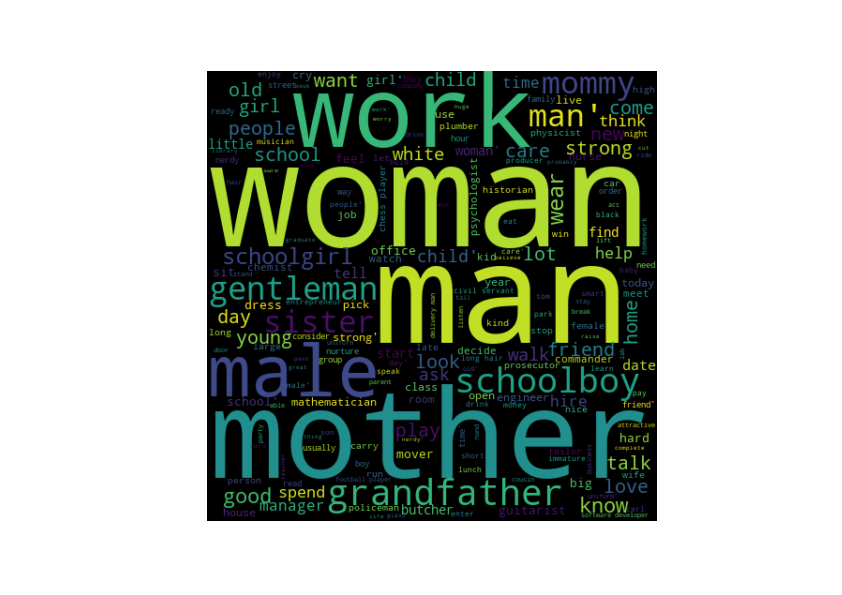
\includegraphics[width=1\textwidth]{thesis/figures/gender.png}
%     \caption{Word cloud  for gender bias type}
%     \label{fig:plural_nouns}
% \end{figure}

% \pagebreak
\begin{figure}
\centering
\begin{minipage}{.5\textwidth}
  \centering
      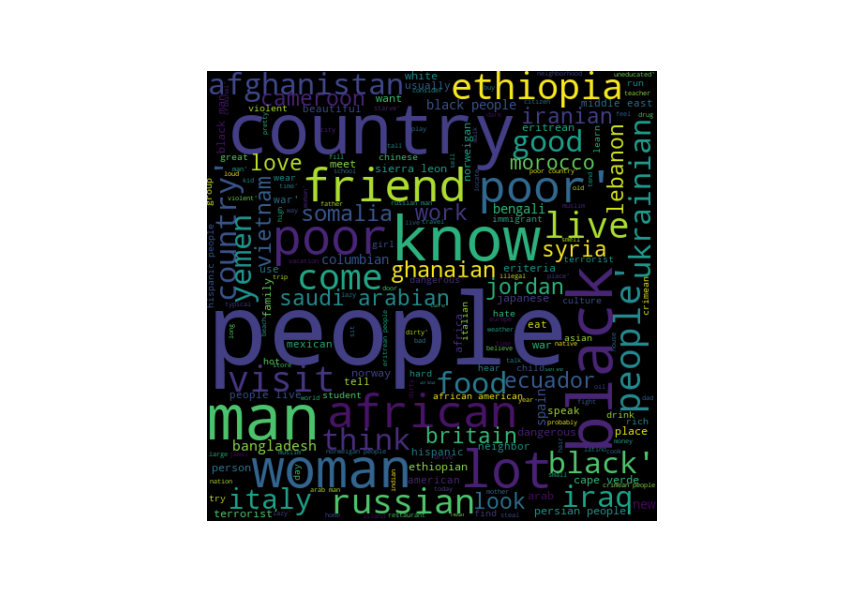
\includegraphics[width=1\textwidth]{thesis/figures/Ethnicity.png}
    \caption{Word cloud for ethnicity bias type}
  \label{fig:test1}
\end{minipage}%
\begin{minipage}{.5\textwidth}
  \centering
    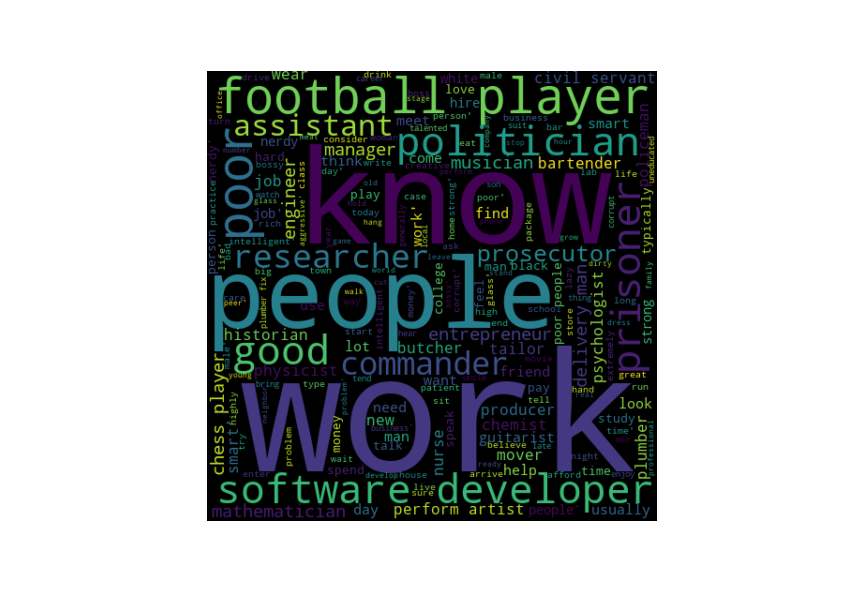
\includegraphics[width=1\textwidth]{thesis/figures/profession.png}
    \caption{Word cloud  for profession bias type}
  \label{fig:test2}
\end{minipage}
\end{figure}

\begin{figure}
\centering
\begin{minipage}{.5\textwidth}
  \centering
    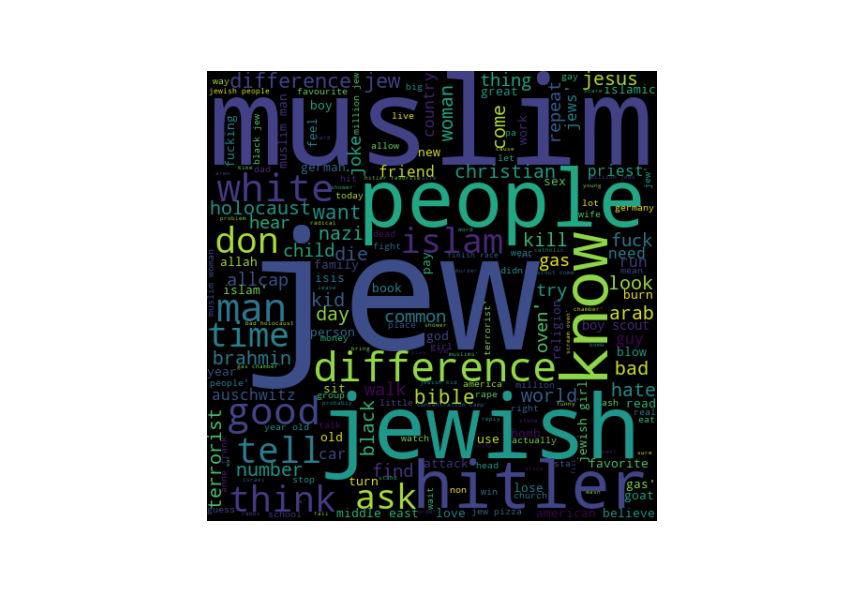
\includegraphics[width=1\textwidth]{thesis/figures/religion.png}
    \caption{Word cloud for religion bias type}
  \label{fig:test1}
\end{minipage}%
\begin{minipage}{.5\textwidth}
  \centering
    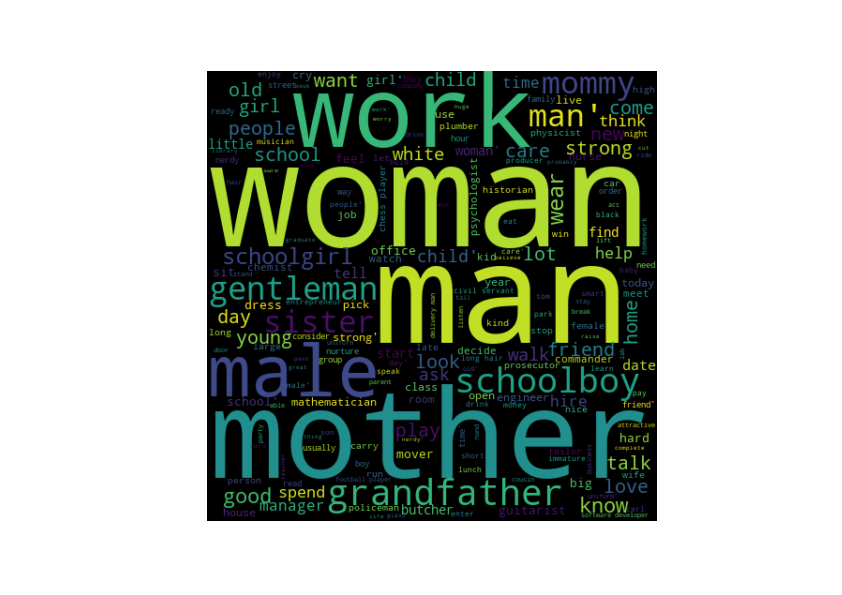
\includegraphics[width=1\textwidth]{thesis/figures/gender.png}
    \caption{Word cloud  for gender bias type}
  \label{fig:test2}
\end{minipage}
\end{figure}

\pagebreak
\subsection{Characteristic attribute terms per bias type}



\subsubsection{Ethnicity}
\subsubsection{Profession}
\subsubsection{Religion}
\subsubsection{Gender}
\section{Lexicons distribution}

\begin{figure}[h!]
\centering
\begin{minipage}{.5\textwidth}
  \centering
      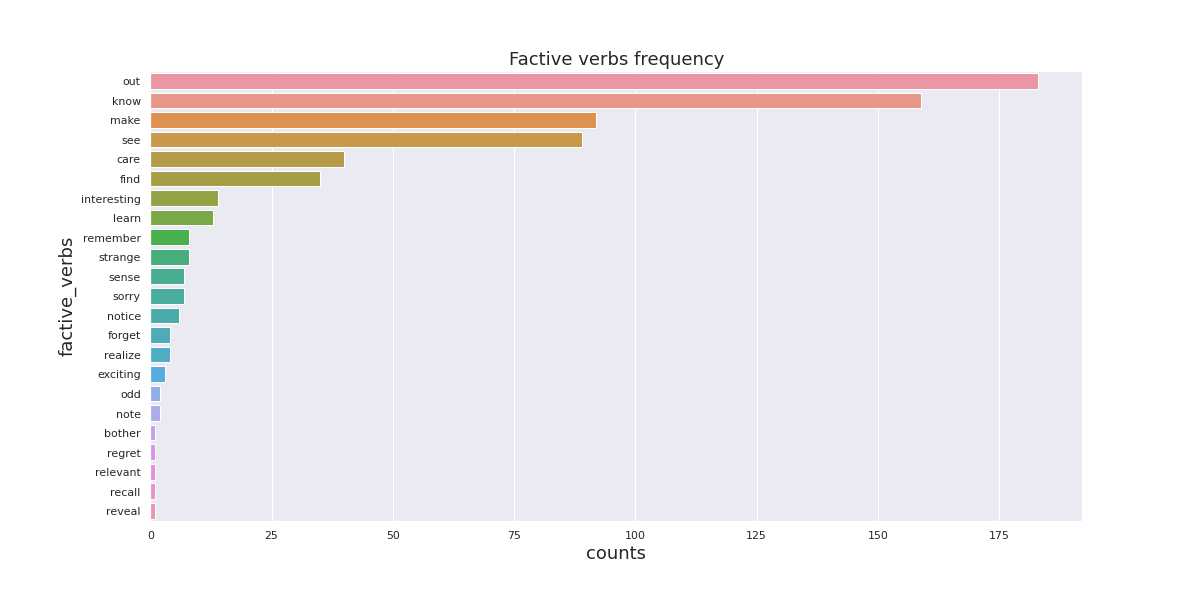
\includegraphics[width=1\textwidth]{thesis/figures/lexicons/LexiconsFactive verbs frequency.png}
    \caption{Factive verbs distribution}
  \label{fig:test1}
\end{minipage}%
\begin{minipage}{.5\textwidth}
  \centering
    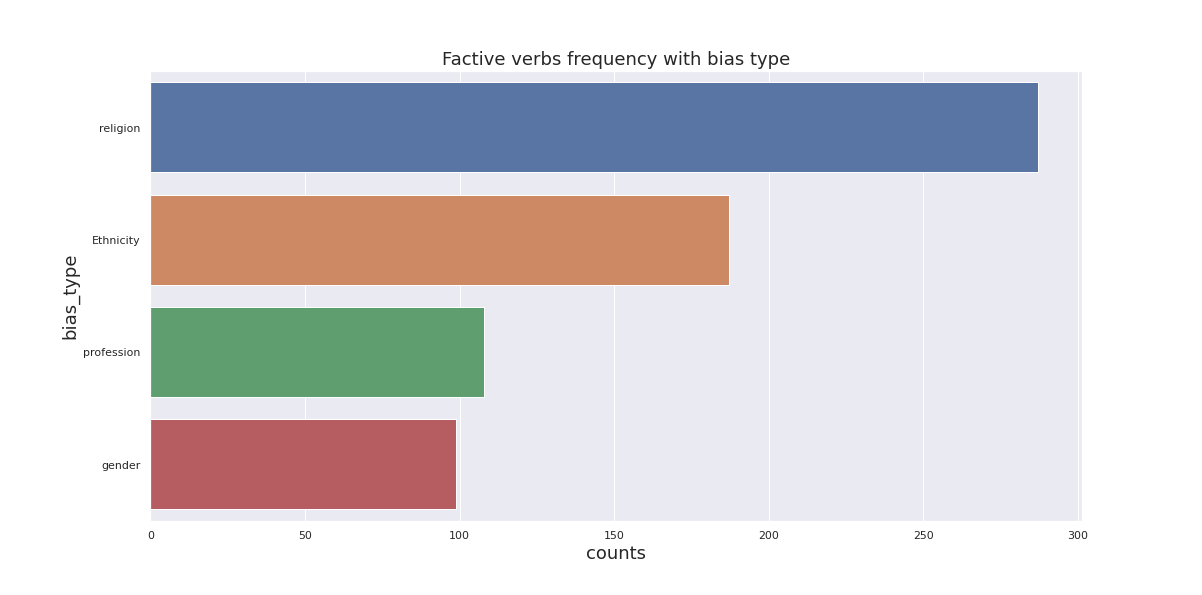
\includegraphics[width=1\textwidth]{thesis/figures/lexicons/LexiconsFactive verbs frequency with bias type.png}
    \caption{Factive words distribution over bias types}
  \label{fig:test2}
\end{minipage}
\end{figure}

\begin{figure}[h!]
\centering
\begin{minipage}{.5\textwidth}
  \centering
      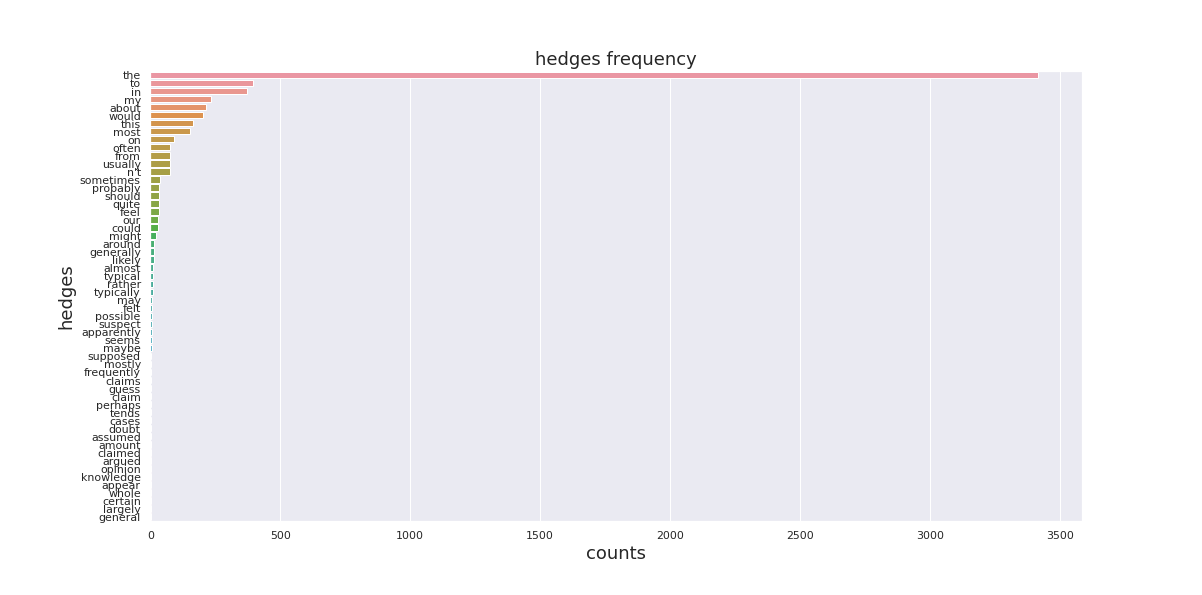
\includegraphics[width=1\textwidth]{thesis/figures/lexicons/Lexiconshedges frequency.png}
    \caption{ Hedges distribution}
  \label{fig:test1}
\end{minipage}%
\begin{minipage}{.5\textwidth}
  \centering
    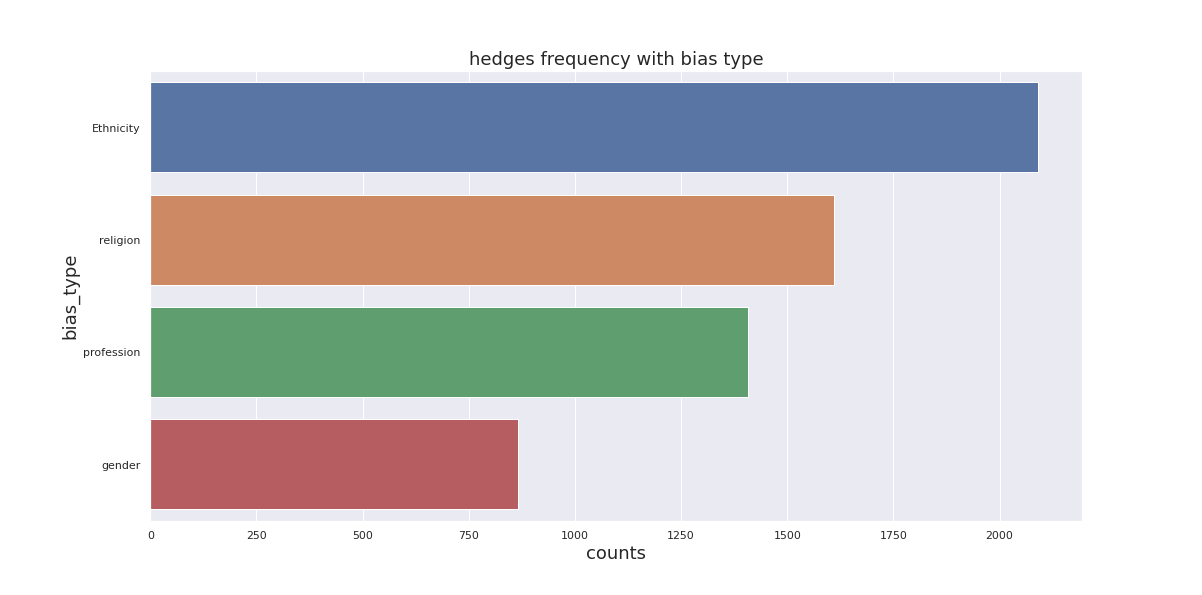
\includegraphics[width=1\textwidth]{thesis/figures/lexicons/Lexiconshedges frequency with bias type.png}
    \caption{Hedge words distribution over bias types}
  \label{fig:test2}
\end{minipage}
\end{figure}

\begin{figure}[h!]
\centering
\begin{minipage}{.5\textwidth}
  \centering
      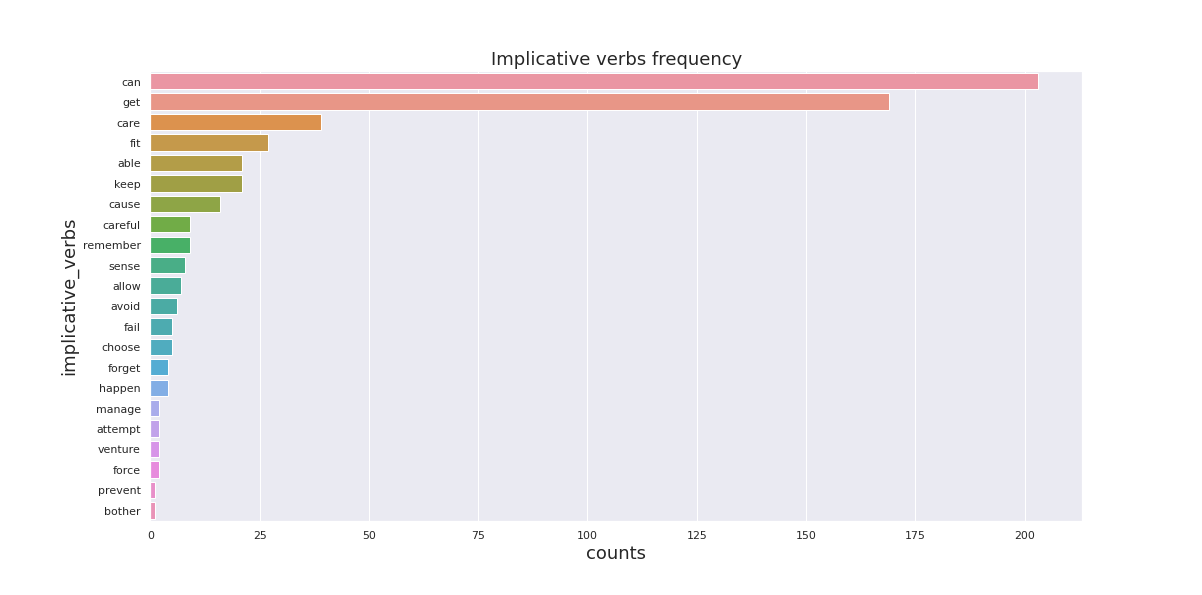
\includegraphics[width=1\textwidth]{thesis/figures/lexicons/LexiconsImplicative verbs frequency.png}
    \caption{ Implicative verbs distribution}
  \label{fig:test1}
\end{minipage}%
\begin{minipage}{.5\textwidth}
  \centering
    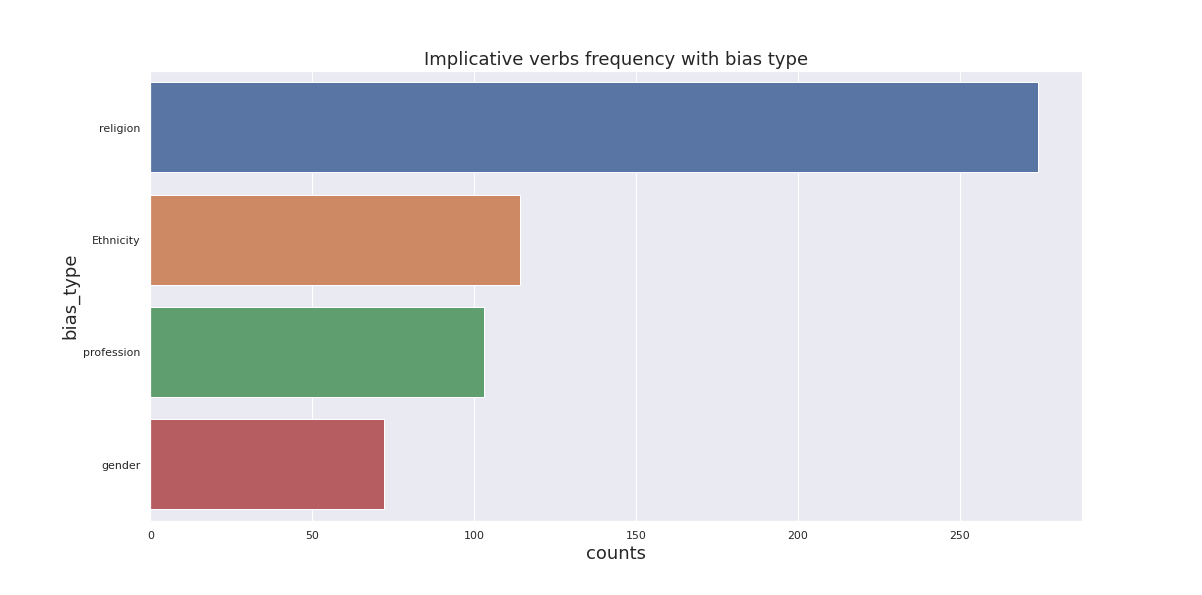
\includegraphics[width=1\textwidth]{thesis/figures/lexicons/LexiconsImplicative verbs frequency with bias type.png}
    \caption{Implicative verbs distribution over bias types}
  \label{fig:test2}
\end{minipage}
\end{figure}

\begin{figure}[h!]
\centering
\begin{minipage}{.5\textwidth}
  \centering
      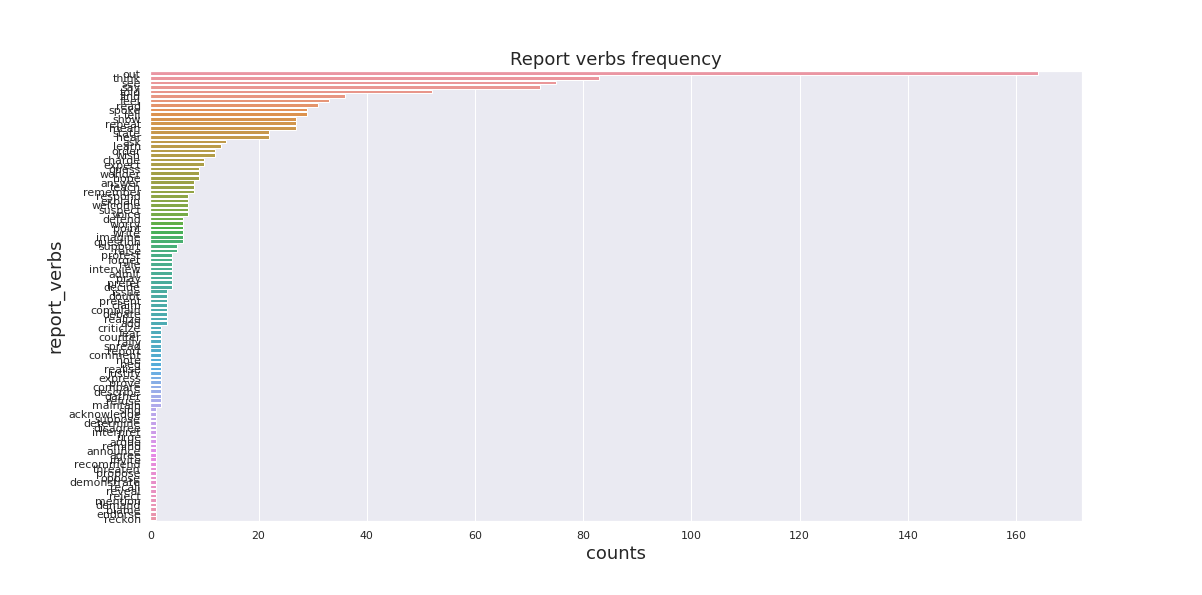
\includegraphics[width=1\textwidth]{thesis/figures/lexicons/LexiconsReport verbs frequency.png}
    \caption{ Report verbs distribution}
  \label{fig:test1}
\end{minipage}%
\begin{minipage}{.5\textwidth}
  \centering
    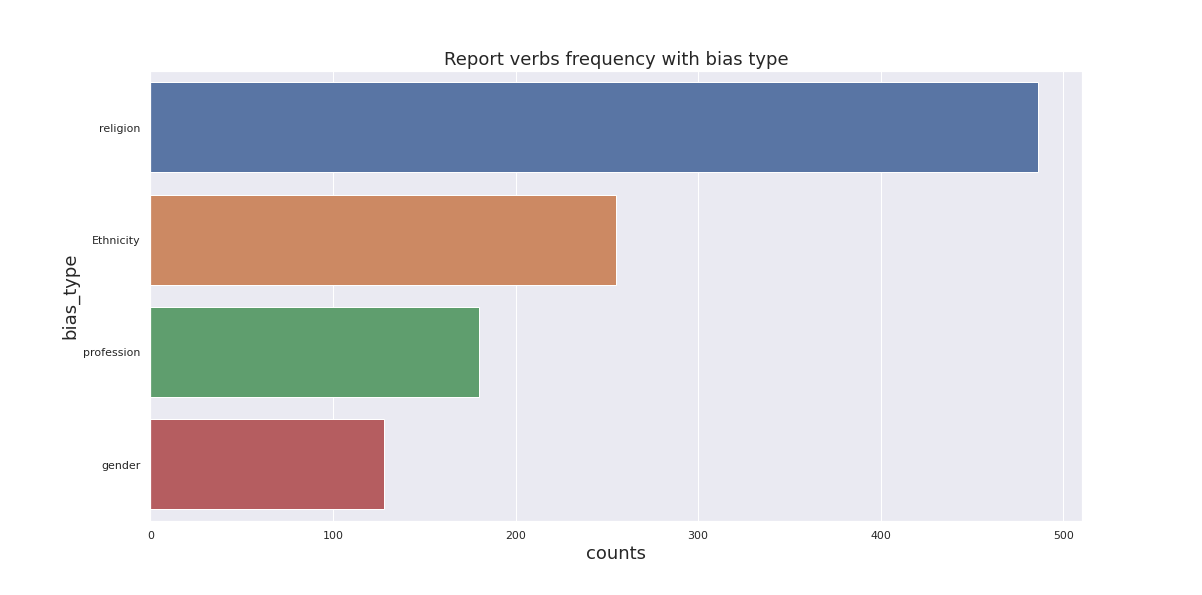
\includegraphics[width=1\textwidth]{thesis/figures/lexicons/LexiconsReport verbs frequency with bias type.png}
    \caption{Report verbs distribution over bias types}
  \label{fig:test2}
\end{minipage}
\end{figure}
\pagebreak
\section{Language Model reports}

% \subsection{Language model hyperparameters}

% \begin{table}[h!]
% \resizebox{\columnwidth}{!}{%
% \begin{tabular}{@{}cccccc@{}}
% \toprule
%   & model\_name       & learning\_rate        & num\_train\_epochs & seed & per\_device\_train\_batch\_size \\ \midrule
%  & roberta-base     & 3.404460046972836e-05 & 5                 & 22   & 8                               \\
%  & xlnet-base-cased  & 2.49816047538945e-05  & 2                  & 15   & 32                              \\
%  & bert-base-uncased & 2.49816047538945e-05  & 2                  & 15   & 32                              \\
%  & gpt2              & 2.49816047538945e-05  & 2                  & 15   & 32                              \\ \bottomrule
% \end{tabular}
% }
% \caption{Hyperparameters used for training language models}
% \label{table:1}
% \end{table}


% Please add the following required packages to your document preamble:
% \usepackage{booktabs}
% \usepackage{multirow}
% \usepackage{graphicx}
% \usepackage{lscape}
\pagebreak
\begin{landscape}
\begin{table}[]
\subsection{Label-wise results}
\resizebox{\columnwidth}{!}{%
\begin{tabular}{@{}lllllllll@{}}
\toprule
Model\_name &
  Metrics &
  Ethnicity &
  Gender &
  Profession &
  Religion &
  Anti-stereotype &
  Stereotype &
  Unrelated \\ \midrule
\multicolumn{1}{|l|}{\multirow{4}{*}{bert\_base\_uncased}} &
  \multicolumn{1}{l|}{precision} &
  \multicolumn{1}{l|}{0.9773299748110831} &
  \multicolumn{1}{l|}{0.8960573476702509} &
  \multicolumn{1}{l|}{0.9004149377593361} &
  \multicolumn{1}{l|}{0.9897610921501706} &
  \multicolumn{1}{l|}{0.6714490674318508} &
  \multicolumn{1}{l|}{0.7202680067001676} &
  \multicolumn{1}{l|}{0.9935064935064936} \\ \cmidrule(l){2-9} 
\multicolumn{1}{|l|}{} &
  \multicolumn{1}{l|}{recall} &
  \multicolumn{1}{l|}{0.9897959183673469} &
  \multicolumn{1}{l|}{0.8223684210526315} &
  \multicolumn{1}{l|}{0.9293361884368309} &
  \multicolumn{1}{l|}{0.9897610921501706} &
  \multicolumn{1}{l|}{0.6015424164524421} &
  \multicolumn{1}{l|}{0.8037383177570093} &
  \multicolumn{1}{l|}{0.9622641509433962} \\ \cmidrule(l){2-9} 
\multicolumn{1}{|l|}{} &
  \multicolumn{1}{l|}{f1-score} &
  \multicolumn{1}{l|}{0.9835234474017743} &
  \multicolumn{1}{l|}{0.8576329331046311} &
  \multicolumn{1}{l|}{0.9146469968387777} &
  \multicolumn{1}{l|}{0.9897610921501706} &
  \multicolumn{1}{l|}{0.6345762711864408} &
  \multicolumn{1}{l|}{0.7597173144876326} &
  \multicolumn{1}{l|}{0.9776357827476039} \\ \cmidrule(l){2-9} 
\multicolumn{1}{|l|}{} &
  \multicolumn{1}{l|}{support} &
  \multicolumn{1}{l|}{784.0} &
  \multicolumn{1}{l|}{304.0} &
  \multicolumn{1}{l|}{467.0} &
  \multicolumn{1}{l|}{293.0} &
  \multicolumn{1}{l|}{778.0} &
  \multicolumn{1}{l|}{1070.0} &
  \multicolumn{1}{l|}{636.0} \\ \midrule
\multicolumn{1}{|l|}{\multirow{4}{*}{roberta-base}} &
  \multicolumn{1}{l|}{precision} &
  \multicolumn{1}{l|}{0.9834394904458599} &
  \multicolumn{1}{l|}{0.8778135048231511} &
  \multicolumn{1}{l|}{0.9261603375527426} &
  \multicolumn{1}{l|}{0.9931740614334471} &
  \multicolumn{1}{l|}{0.7858176555716353} &
  \multicolumn{1}{l|}{0.8038194444444444} &
  \multicolumn{1}{l|}{0.9935587761674718} \\ \cmidrule(l){2-9} 
\multicolumn{1}{|l|}{} &
  \multicolumn{1}{l|}{recall} &
  \multicolumn{1}{l|}{0.9846938775510204} &
  \multicolumn{1}{l|}{0.8980263157894737} &
  \multicolumn{1}{l|}{0.9400428265524625} &
  \multicolumn{1}{l|}{0.9931740614334471} &
  \multicolumn{1}{l|}{0.6979434447300771} &
  \multicolumn{1}{l|}{0.8654205607476636} &
  \multicolumn{1}{l|}{0.970125786163522} \\ \cmidrule(l){2-9} 
\multicolumn{1}{|l|}{} &
  \multicolumn{1}{l|}{f1-score} &
  \multicolumn{1}{l|}{0.9840662842574888} &
  \multicolumn{1}{l|}{0.8878048780487804} &
  \multicolumn{1}{l|}{0.9330499468650373} &
  \multicolumn{1}{l|}{0.9931740614334471} &
  \multicolumn{1}{l|}{0.7392784206943499} &
  \multicolumn{1}{l|}{0.8334833483348336} &
  \multicolumn{1}{l|}{0.9817024661893397} \\ \cmidrule(l){2-9} 
\multicolumn{1}{|l|}{} &
  \multicolumn{1}{l|}{support} &
  \multicolumn{1}{l|}{784.0} &
  \multicolumn{1}{l|}{304.0} &
  \multicolumn{1}{l|}{467.0} &
  \multicolumn{1}{l|}{293.0} &
  \multicolumn{1}{l|}{778.0} &
  \multicolumn{1}{l|}{1070.0} &
  \multicolumn{1}{l|}{636.0} \\ \midrule
\multicolumn{1}{|l|}{\multirow{4}{*}{xlnet-base-cased}} &
  \multicolumn{1}{l|}{precision} &
  \multicolumn{1}{l|}{0.96625} &
  \multicolumn{1}{l|}{0.8951310861423221} &
  \multicolumn{1}{l|}{0.9014989293361885} &
  \multicolumn{1}{l|}{0.993103448275862} &
  \multicolumn{1}{l|}{0.8062015503875969} &
  \multicolumn{1}{l|}{0.8386699507389163} &
  \multicolumn{1}{l|}{0.9916943521594684} \\ \cmidrule(l){2-9} 
\multicolumn{1}{|l|}{} &
  \multicolumn{1}{l|}{recall} &
  \multicolumn{1}{l|}{0.985969387755102} &
  \multicolumn{1}{l|}{0.7861842105263158} &
  \multicolumn{1}{l|}{0.9014989293361885} &
  \multicolumn{1}{l|}{0.9829351535836177} &
  \multicolumn{1}{l|}{0.40102827763496146} &
  \multicolumn{1}{l|}{0.6364485981308411} &
  \multicolumn{1}{l|}{0.9386792452830188} \\ \cmidrule(l){2-9} 
\multicolumn{1}{|l|}{} &
  \multicolumn{1}{l|}{f1-score} &
  \multicolumn{1}{l|}{0.9760101010101009} &
  \multicolumn{1}{l|}{0.8371278458844135} &
  \multicolumn{1}{l|}{0.9014989293361885} &
  \multicolumn{1}{l|}{0.9879931389365352} &
  \multicolumn{1}{l|}{0.5356223175965665} &
  \multicolumn{1}{l|}{0.7236981934112645} &
  \multicolumn{1}{l|}{0.9644588045234248} \\ \cmidrule(l){2-9} 
\multicolumn{1}{|l|}{} &
  \multicolumn{1}{l|}{support} &
  \multicolumn{1}{l|}{784.0} &
  \multicolumn{1}{l|}{304.0} &
  \multicolumn{1}{l|}{467.0} &
  \multicolumn{1}{l|}{293.0} &
  \multicolumn{1}{l|}{778.0} &
  \multicolumn{1}{l|}{1070.0} &
  \multicolumn{1}{l|}{636.0} \\ \midrule
\multicolumn{1}{|l|}{\multirow{4}{*}{gpt2}} &
  \multicolumn{1}{l|}{precision} &
  \multicolumn{1}{l|}{0.9219178082191781} &
  \multicolumn{1}{l|}{0.8918918918918919} &
  \multicolumn{1}{l|}{0.8039647577092511} &
  \multicolumn{1}{l|}{0.9745454545454545} &
  \multicolumn{1}{l|}{0.5833333333333334} &
  \multicolumn{1}{l|}{0.8333333333333334} &
  \multicolumn{1}{l|}{0.9515260323159784} \\ \cmidrule(l){2-9} 
\multicolumn{1}{|l|}{} &
  \multicolumn{1}{l|}{recall} &
  \multicolumn{1}{l|}{0.8584183673469388} &
  \multicolumn{1}{l|}{0.4342105263157895} &
  \multicolumn{1}{l|}{0.7815845824411135} &
  \multicolumn{1}{l|}{0.9146757679180887} &
  \multicolumn{1}{l|}{0.12596401028277635} &
  \multicolumn{1}{l|}{0.3317757009345794} &
  \multicolumn{1}{l|}{0.8333333333333334} \\ \cmidrule(l){2-9} 
\multicolumn{1}{|l|}{} &
  \multicolumn{1}{l|}{f1-score} &
  \multicolumn{1}{l|}{0.8890356671070013} &
  \multicolumn{1}{l|}{0.5840707964601769} &
  \multicolumn{1}{l|}{0.7926167209554832} &
  \multicolumn{1}{l|}{0.9436619718309859} &
  \multicolumn{1}{l|}{0.20718816067653276} &
  \multicolumn{1}{l|}{0.4745989304812835} &
  \multicolumn{1}{l|}{0.8885163453478626} \\ \cmidrule(l){2-9} 
\multicolumn{1}{|l|}{} &
  \multicolumn{1}{l|}{support} &
  \multicolumn{1}{l|}{784.0} &
  \multicolumn{1}{l|}{304.0} &
  \multicolumn{1}{l|}{467.0} &
  \multicolumn{1}{l|}{293.0} &
  \multicolumn{1}{l|}{778.0} &
  \multicolumn{1}{l|}{1070.0} &
  \multicolumn{1}{l|}{636.0} \\ \bottomrule
\end{tabular}%
}
\caption{Label wise precision, recall, f1score and support measures}
\label{tab:Per-Label-precision-recall-f-measure}
\end{table}
\end{landscape}

\section{Baseline reports}

\subsection{Label-wise results}
\subsubsection{Label-wise CNN}
% Please add the following required packages to your document preamble:
% \usepackage{booktabs}
% \usepackage{multirow}
% \usepackage{graphicx}
\begin{table}[h!]
\resizebox{\textwidth}{!}{%
\begin{tabular}{@{}clllllllll@{}}
\toprule
\multicolumn{1}{l}{Model name} &
  Text features &
  Metrics &
  Ethnicity &
  gender &
  profession &
  religion &
  Anti-stereotype &
  stereotype &
  unrelated \\ \midrule
\multicolumn{1}{|c|}{\multirow{4}{*}{CNN}} &
  \multicolumn{1}{c|}{\multirow{4}{*}{Flair word embedding}} &
  \multicolumn{1}{l|}{precision} &
  \multicolumn{1}{l|}{0.5289421157684631} &
  \multicolumn{1}{l|}{0.22929936305732485} &
  \multicolumn{1}{l|}{0.422360248447205} &
  \multicolumn{1}{l|}{0.5942857142857143} &
  \multicolumn{1}{l|}{0.43267776096822996} &
  \multicolumn{1}{l|}{0.6020278833967047} &
  \multicolumn{1}{l|}{0.4857142857142857} \\ \cmidrule(l){3-10} 
\multicolumn{1}{|c|}{} &
  \multicolumn{1}{c|}{} &
  \multicolumn{1}{l|}{recall} &
  \multicolumn{1}{l|}{0.3380102040816326} &
  \multicolumn{1}{l|}{0.23684210526315788} &
  \multicolumn{1}{l|}{0.291220556745182} &
  \multicolumn{1}{l|}{0.7098976109215017} &
  \multicolumn{1}{l|}{0.3676092544987147} &
  \multicolumn{1}{l|}{0.4439252336448598} &
  \multicolumn{1}{l|}{0.6949685534591195} \\ \cmidrule(l){3-10} 
\multicolumn{1}{|c|}{} &
  \multicolumn{1}{c|}{} &
  \multicolumn{1}{l|}{f1-score} &
  \multicolumn{1}{l|}{0.41245136186770426} &
  \multicolumn{1}{l|}{0.23300970873786406} &
  \multicolumn{1}{l|}{0.3447401774397972} &
  \multicolumn{1}{l|}{0.6469673405909798} &
  \multicolumn{1}{l|}{0.3974982626824184} &
  \multicolumn{1}{l|}{0.5110274341043572} &
  \multicolumn{1}{l|}{0.5717981888745148} \\ \cmidrule(l){3-10} 
\multicolumn{1}{|c|}{} &
  \multicolumn{1}{c|}{} &
  \multicolumn{1}{l|}{support} &
  \multicolumn{1}{l|}{784.0} &
  \multicolumn{1}{l|}{304.0} &
  \multicolumn{1}{l|}{467.0} &
  \multicolumn{1}{l|}{293.0} &
  \multicolumn{1}{l|}{778.0} &
  \multicolumn{1}{l|}{1070.0} &
  \multicolumn{1}{l|}{636.0} \\ \midrule
\multicolumn{1}{|c|}{\multirow{4}{*}{CNN}} &
  \multicolumn{1}{l|}{\multirow{4}{*}{Glove word embedding}} &
  \multicolumn{1}{l|}{precision} &
  \multicolumn{1}{l|}{0.3486238532110092} &
  \multicolumn{1}{l|}{0.11728395061728394} &
  \multicolumn{1}{l|}{0.2716417910447761} &
  \multicolumn{1}{l|}{0.49056603773584906} &
  \multicolumn{1}{l|}{0.4088397790055249} &
  \multicolumn{1}{l|}{0.5549949545913219} &
  \multicolumn{1}{l|}{0.4480651731160896} \\ \cmidrule(l){3-10} 
\multicolumn{1}{|l|}{} &
  \multicolumn{1}{l|}{} &
  \multicolumn{1}{l|}{recall} &
  \multicolumn{1}{l|}{0.2423469387755102} &
  \multicolumn{1}{l|}{0.0625} &
  \multicolumn{1}{l|}{0.1948608137044968} &
  \multicolumn{1}{l|}{0.5324232081911263} &
  \multicolumn{1}{l|}{0.09511568123393316} &
  \multicolumn{1}{l|}{0.514018691588785} &
  \multicolumn{1}{l|}{0.6918238993710691} \\ \cmidrule(l){3-10} 
\multicolumn{1}{|l|}{} &
  \multicolumn{1}{l|}{} &
  \multicolumn{1}{l|}{f1-score} &
  \multicolumn{1}{l|}{0.28592927012791575} &
  \multicolumn{1}{l|}{0.0815450643776824} &
  \multicolumn{1}{l|}{0.22693266832917708} &
  \multicolumn{1}{l|}{0.5106382978723404} &
  \multicolumn{1}{l|}{0.1543274244004171} &
  \multicolumn{1}{l|}{0.5337214944201845} &
  \multicolumn{1}{l|}{0.5438813349814586} \\ \cmidrule(l){3-10} 
\multicolumn{1}{|l|}{} &
  \multicolumn{1}{l|}{} &
  \multicolumn{1}{l|}{support} &
  \multicolumn{1}{l|}{784.0} &
  \multicolumn{1}{l|}{304.0} &
  \multicolumn{1}{l|}{467.0} &
  \multicolumn{1}{l|}{293.0} &
  \multicolumn{1}{l|}{778.0} &
  \multicolumn{1}{l|}{1070.0} &
  \multicolumn{1}{l|}{636.0} \\ \midrule
\multicolumn{1}{|c|}{\multirow{4}{*}{CNN}} &
  \multicolumn{1}{l|}{\multirow{4}{*}{Fasttext word embedding}} &
  \multicolumn{1}{l|}{precision} &
  \multicolumn{1}{l|}{0.360062893081761} &
  \multicolumn{1}{l|}{0.14067278287461774} &
  \multicolumn{1}{l|}{0.2283464566929134} &
  \multicolumn{1}{l|}{0.4798657718120805} &
  \multicolumn{1}{l|}{0.40894039735099336} &
  \multicolumn{1}{l|}{0.6540178571428571} &
  \multicolumn{1}{l|}{0.49573863636363635} \\ \cmidrule(l){3-10} 
\multicolumn{1}{|c|}{} &
  \multicolumn{1}{l|}{} &
  \multicolumn{1}{l|}{recall} &
  \multicolumn{1}{l|}{0.29209183673469385} &
  \multicolumn{1}{l|}{0.1513157894736842} &
  \multicolumn{1}{l|}{0.18629550321199143} &
  \multicolumn{1}{l|}{0.4880546075085324} &
  \multicolumn{1}{l|}{0.6349614395886889} &
  \multicolumn{1}{l|}{0.2738317757009346} &
  \multicolumn{1}{l|}{0.5487421383647799} \\ \cmidrule(l){3-10} 
\multicolumn{1}{|c|}{} &
  \multicolumn{1}{l|}{} &
  \multicolumn{1}{l|}{f1-score} &
  \multicolumn{1}{l|}{0.3225352112676056} &
  \multicolumn{1}{l|}{0.14580031695721077} &
  \multicolumn{1}{l|}{0.20518867924528303} &
  \multicolumn{1}{l|}{0.4839255499153976} &
  \multicolumn{1}{l|}{0.49748237663645517} &
  \multicolumn{1}{l|}{0.38603425559947296} &
  \multicolumn{1}{l|}{0.5208955223880597} \\ \cmidrule(l){3-10} 
\multicolumn{1}{|c|}{} &
  \multicolumn{1}{l|}{} &
  \multicolumn{1}{l|}{support} &
  \multicolumn{1}{l|}{784.0} &
  \multicolumn{1}{l|}{304.0} &
  \multicolumn{1}{l|}{467.0} &
  \multicolumn{1}{l|}{293.0} &
  \multicolumn{1}{l|}{778.0} &
  \multicolumn{1}{l|}{1070.0} &
  \multicolumn{1}{l|}{636.0} \\ \bottomrule
\end{tabular}%
}
\caption{Label-wise scores of CNN models}
\label{tab:Label-wise-CNN}
\end{table}

\subsubsection{Label-wise MNB}
% Please add the following required packages to your document preamble:
% \usepackage{booktabs}
% \usepackage{multirow}
% \usepackage{graphicx}
\begin{table}[h!]
\resizebox{\textwidth}{!}{%
\begin{tabular}{@{}ccllllllll@{}}
\toprule
\multicolumn{1}{l}{Model name} &
  \multicolumn{1}{l}{Text feature} &
  Metrics &
  Ethnicity &
  gender &
  profession &
  religion &
  Anti-stereotype &
  stereotype &
  unrelated \\ \midrule
\multicolumn{1}{|c|}{\multirow{4}{*}{MNB}} &
  \multicolumn{1}{c|}{\multirow{4}{*}{Bow}} &
  \multicolumn{1}{l|}{precision} &
  \multicolumn{1}{l|}{0.8687116564417178} &
  \multicolumn{1}{l|}{0.6818181818181818} &
  \multicolumn{1}{l|}{0.780439121756487} &
  \multicolumn{1}{l|}{0.8597122302158273} &
  \multicolumn{1}{l|}{0.49623250807319697} &
  \multicolumn{1}{l|}{0.6677524429967426} &
  \multicolumn{1}{l|}{0.9606003752345216} \\ \cmidrule(l){3-10} 
\multicolumn{1}{|c|}{} &
  \multicolumn{1}{c|}{} &
  \multicolumn{1}{l|}{recall} &
  \multicolumn{1}{l|}{0.9030612244897959} &
  \multicolumn{1}{l|}{0.6435643564356436} &
  \multicolumn{1}{l|}{0.8372591006423983} &
  \multicolumn{1}{l|}{0.8156996587030717} &
  \multicolumn{1}{l|}{0.5933075933075933} &
  \multicolumn{1}{l|}{0.5747663551401869} &
  \multicolumn{1}{l|}{0.8037676609105181} \\ \cmidrule(l){3-10} 
\multicolumn{1}{|c|}{} &
  \multicolumn{1}{c|}{} &
  \multicolumn{1}{l|}{f1-score} &
  \multicolumn{1}{l|}{0.8855534709193245} &
  \multicolumn{1}{l|}{0.6621392190152802} &
  \multicolumn{1}{l|}{0.8078512396694214} &
  \multicolumn{1}{l|}{0.8371278458844134} &
  \multicolumn{1}{l|}{0.540445486518171} &
  \multicolumn{1}{l|}{0.6177800100452036} &
  \multicolumn{1}{l|}{0.8752136752136753} \\ \cmidrule(l){3-10} 
\multicolumn{1}{|c|}{} &
  \multicolumn{1}{c|}{} &
  \multicolumn{1}{l|}{support} &
  \multicolumn{1}{l|}{784.0} &
  \multicolumn{1}{l|}{303.0} &
  \multicolumn{1}{l|}{467.0} &
  \multicolumn{1}{l|}{293.0} &
  \multicolumn{1}{l|}{777.0} &
  \multicolumn{1}{l|}{1070.0} &
  \multicolumn{1}{l|}{637.0} \\ \midrule
\multicolumn{1}{|c|}{\multirow{4}{*}{MNB}} &
  \multicolumn{1}{c|}{\multirow{4}{*}{Tf\_idf}} &
  \multicolumn{1}{l|}{precision} &
  \multicolumn{1}{l|}{0.9517884914463453} &
  \multicolumn{1}{l|}{0.975} &
  \multicolumn{1}{l|}{0.8913043478260869} &
  \multicolumn{1}{l|}{1.0} &
  \multicolumn{1}{l|}{0.49019607843137253} &
  \multicolumn{1}{l|}{0.725094577553594} &
  \multicolumn{1}{l|}{0.979539641943734} \\ \cmidrule(l){3-10} 
\multicolumn{1}{|c|}{} &
  \multicolumn{1}{c|}{} &
  \multicolumn{1}{l|}{recall} &
  \multicolumn{1}{l|}{0.7806122448979592} &
  \multicolumn{1}{l|}{0.12871287128712872} &
  \multicolumn{1}{l|}{0.43897216274089934} &
  \multicolumn{1}{l|}{0.4300341296928328} &
  \multicolumn{1}{l|}{0.16087516087516088} &
  \multicolumn{1}{l|}{0.5373831775700935} &
  \multicolumn{1}{l|}{0.6012558869701727} \\ \cmidrule(l){3-10} 
\multicolumn{1}{|c|}{} &
  \multicolumn{1}{c|}{} &
  \multicolumn{1}{l|}{f1-score} &
  \multicolumn{1}{l|}{0.8577435178696567} &
  \multicolumn{1}{l|}{0.2274052478134111} &
  \multicolumn{1}{l|}{0.5882352941176471} &
  \multicolumn{1}{l|}{0.6014319809069213} &
  \multicolumn{1}{l|}{0.24224806201550386} &
  \multicolumn{1}{l|}{0.6172839506172839} &
  \multicolumn{1}{l|}{0.7451361867704281} \\ \cmidrule(l){3-10} 
\multicolumn{1}{|c|}{} &
  \multicolumn{1}{c|}{} &
  \multicolumn{1}{l|}{support} &
  \multicolumn{1}{l|}{784.0} &
  \multicolumn{1}{l|}{303.0} &
  \multicolumn{1}{l|}{467.0} &
  \multicolumn{1}{l|}{293.0} &
  \multicolumn{1}{l|}{777.0} &
  \multicolumn{1}{l|}{1070.0} &
  \multicolumn{1}{l|}{637.0} \\ \bottomrule
\end{tabular}%
}
\caption{Label-wise scores of Multinomial Naive Bayes}
\label{tab:Label-wise-Naiye-Bayes}
\end{table}

\subsubsection{Label-wise KNN}
% Please add the following required packages to your document preamble:
% \usepackage{booktabs}
% \usepackage{multirow}
% \usepackage{graphicx}
\begin{table}[h!]
\resizebox{\textwidth}{!}{%
\begin{tabular}{@{}|c|c|l|l|l|l|l|l|l|l|@{}}
\toprule
\multicolumn{1}{|l|}{Model name} &
  \multicolumn{1}{l|}{Text features} &
  Metrics &
  Ethnicity &
  gender &
  profession &
  religion &
  Anti-stereotype &
  stereotype &
  unrelated \\ \midrule
\multirow{4}{*}{KNN} &
  \multirow{4}{*}{Bow} &
  precision &
  0.8491295938104448 &
  0.795774647887324 &
  0.7058823529411765 &
  0.9882352941176471 &
  0.34615384615384615 &
  0.48523206751054854 &
  0.5892661555312158 \\ \cmidrule(l){3-10} 
 &
   &
  recall &
  0.5599489795918368 &
  0.37293729372937295 &
  0.5910064239828694 &
  0.28668941979522183 &
  0.18532818532818532 &
  0.32242990654205606 &
  0.8445839874411303 \\ \cmidrule(l){3-10} 
 &
   &
  f1-score &
  0.6748654880860876 &
  0.507865168539326 &
  0.6433566433566433 &
  0.4444444444444444 &
  0.24140821458507963 &
  0.38742279618192027 &
  0.6941935483870967 \\ \cmidrule(l){3-10} 
 &
   &
  support &
  784.0 &
  303.0 &
  467.0 &
  293.0 &
  777.0 &
  1070.0 &
  637.0 \\ \midrule
\multirow{4}{*}{KNN} &
  \multirow{4}{*}{Tf\_idf} &
  precision &
  0.9503105590062112 &
  0.5503355704697986 &
  0.9021739130434783 &
  0.9791666666666666 &
  0.2863070539419087 &
  0.7008928571428571 &
  0.3486646884272997 \\ \cmidrule(l){3-10} 
 &
   &
  recall &
  0.1951530612244898 &
  0.2706270627062706 &
  0.1777301927194861 &
  0.16040955631399317 &
  0.0888030888030888 &
  0.14672897196261683 &
  0.7378335949764521 \\ \cmidrule(l){3-10} 
 &
   &
  f1-score &
  0.3238095238095238 &
  0.36283185840707965 &
  0.29695885509839 &
  0.2756598240469208 &
  0.13555992141453832 &
  0.24265842349304484 &
  0.473551637279597 \\ \cmidrule(l){3-10} 
 &
   &
  support &
  784.0 &
  303.0 &
  467.0 &
  293.0 &
  777.0 &
  1070.0 &
  637.0 \\ \bottomrule
\end{tabular}%
}
\caption{Label-wise scores of k-nearest neighbors}
\label{tab:Label-wise-KNN}
\end{table}
\subsubsection{Label-wise SVM with selected features}
% Please add the following required packages to your document preamble:
% \usepackage{booktabs}
% \usepackage{multirow}
% \usepackage{graphicx}
\begin{table}[h!]
\resizebox{\textwidth}{!}{%
\begin{tabular}{@{}clllllllll@{}}
\toprule
\multicolumn{1}{l}{Model name} &
  Text features &
  Metrics &
  Ethnicity &
  gender &
  profession &
  religion &
  Anti-stereotype &
  stereotype &
  unrelated \\ \midrule
\multicolumn{1}{|c|}{\multirow{4}{*}{SVM}} &
  \multicolumn{1}{l|}{\multirow{4}{*}{Selected features}} &
  \multicolumn{1}{l|}{precision} &
  \multicolumn{1}{l|}{0.8231098430813124} &
  \multicolumn{1}{l|}{0.8421052631578947} &
  \multicolumn{1}{l|}{0.7664670658682635} &
  \multicolumn{1}{l|}{0.8592964824120602} &
  \multicolumn{1}{l|}{0.0} &
  \multicolumn{1}{l|}{0.6795665634674922} &
  \multicolumn{1}{l|}{0.7216117216117216} \\ \cmidrule(l){3-10} 
\multicolumn{1}{|c|}{} &
  \multicolumn{1}{l|}{} &
  \multicolumn{1}{l|}{recall} &
  \multicolumn{1}{l|}{0.735969387755102} &
  \multicolumn{1}{l|}{0.15841584158415842} &
  \multicolumn{1}{l|}{0.5481798715203426} &
  \multicolumn{1}{l|}{0.5836177474402731} &
  \multicolumn{1}{l|}{0.0} &
  \multicolumn{1}{l|}{0.4102803738317757} &
  \multicolumn{1}{l|}{0.6185243328100472} \\ \cmidrule(l){3-10} 
\multicolumn{1}{|c|}{} &
  \multicolumn{1}{l|}{} &
  \multicolumn{1}{l|}{f1-score} &
  \multicolumn{1}{l|}{0.7771043771043771} &
  \multicolumn{1}{l|}{0.26666666666666666} &
  \multicolumn{1}{l|}{0.6392009987515607} &
  \multicolumn{1}{l|}{0.6951219512195121} &
  \multicolumn{1}{l|}{0.0} &
  \multicolumn{1}{l|}{0.5116550116550116} &
  \multicolumn{1}{l|}{0.6661031276415893} \\ \cmidrule(l){3-10} 
\multicolumn{1}{|c|}{} &
  \multicolumn{1}{l|}{} &
  \multicolumn{1}{l|}{support} &
  \multicolumn{1}{l|}{784.0} &
  \multicolumn{1}{l|}{303.0} &
  \multicolumn{1}{l|}{467.0} &
  \multicolumn{1}{l|}{293.0} &
  \multicolumn{1}{l|}{777.0} &
  \multicolumn{1}{l|}{1070.0} &
  \multicolumn{1}{l|}{637.0} \\ \bottomrule
\end{tabular}%
}
\caption{Label-wise scores with SVM with selected features}
\label{tab:Label-wise-SVM}
\end{table}

\pagebreak

\subsubsection{Label-wise Random forest}
% Please add the following required packages to your document preamble:
% \usepackage{booktabs}
% \usepackage{multirow}
% \usepackage{graphicx}
\begin{table}[h!]
\resizebox{\textwidth}{!}{%
\begin{tabular}{@{}ccllllllll@{}}
\toprule
\multicolumn{1}{l}{Model name} &
  \multicolumn{1}{l}{Text feature} &
  Metrics &
  Ethnicity &
  gender &
  profession &
  religion &
  Anti-stereotype &
  stereotype &
  unrelated \\ \midrule
\multicolumn{1}{|c|}{\multirow{4}{*}{RandomForest\_bow}} &
  \multicolumn{1}{c|}{\multirow{4}{*}{Bow}} &
  \multicolumn{1}{l|}{precision} &
  \multicolumn{1}{l|}{0.9334389857369255} &
  \multicolumn{1}{l|}{0.9577464788732394} &
  \multicolumn{1}{l|}{0.9550173010380623} &
  \multicolumn{1}{l|}{0.9875} &
  \multicolumn{1}{l|}{0.2737819025522042} &
  \multicolumn{1}{l|}{0.5189873417721519} &
  \multicolumn{1}{l|}{0.9563758389261745} \\ \cmidrule(l){3-10} 
\multicolumn{1}{|c|}{} &
  \multicolumn{1}{c|}{} &
  \multicolumn{1}{l|}{recall} &
  \multicolumn{1}{l|}{0.7512755102040817} &
  \multicolumn{1}{l|}{0.44884488448844884} &
  \multicolumn{1}{l|}{0.5910064239828694} &
  \multicolumn{1}{l|}{0.5392491467576792} &
  \multicolumn{1}{l|}{0.15186615186615188} &
  \multicolumn{1}{l|}{0.38317757009345793} &
  \multicolumn{1}{l|}{0.8948194662480377} \\ \cmidrule(l){3-10} 
\multicolumn{1}{|c|}{} &
  \multicolumn{1}{c|}{} &
  \multicolumn{1}{l|}{f1-score} &
  \multicolumn{1}{l|}{0.8325088339222615} &
  \multicolumn{1}{l|}{0.6112359550561798} &
  \multicolumn{1}{l|}{0.7301587301587302} &
  \multicolumn{1}{l|}{0.6975717439293599} &
  \multicolumn{1}{l|}{0.19536423841059603} &
  \multicolumn{1}{l|}{0.44086021505376344} &
  \multicolumn{1}{l|}{0.9245742092457421} \\ \cmidrule(l){3-10} 
\multicolumn{1}{|c|}{} &
  \multicolumn{1}{c|}{} &
  \multicolumn{1}{l|}{support} &
  \multicolumn{1}{l|}{784.0} &
  \multicolumn{1}{l|}{303.0} &
  \multicolumn{1}{l|}{467.0} &
  \multicolumn{1}{l|}{293.0} &
  \multicolumn{1}{l|}{777.0} &
  \multicolumn{1}{l|}{1070.0} &
  \multicolumn{1}{l|}{637.0} \\ \midrule
\multicolumn{1}{|c|}{\multirow{4}{*}{RandomForest\_tf\_idf}} &
  \multicolumn{1}{c|}{\multirow{4}{*}{Tf\_idf}} &
  \multicolumn{1}{l|}{precision} &
  \multicolumn{1}{l|}{0.9486823855755895} &
  \multicolumn{1}{l|}{0.9512195121951219} &
  \multicolumn{1}{l|}{0.8896882494004796} &
  \multicolumn{1}{l|}{0.9908256880733946} &
  \multicolumn{1}{l|}{0.4063157894736842} &
  \multicolumn{1}{l|}{0.5949074074074074} &
  \multicolumn{1}{l|}{0.911353032659409} \\ \cmidrule(l){3-10} 
\multicolumn{1}{|c|}{} &
  \multicolumn{1}{c|}{} &
  \multicolumn{1}{l|}{recall} &
  \multicolumn{1}{l|}{0.8724489795918368} &
  \multicolumn{1}{l|}{0.5148514851485149} &
  \multicolumn{1}{l|}{0.7944325481798715} &
  \multicolumn{1}{l|}{0.7372013651877133} &
  \multicolumn{1}{l|}{0.2483912483912484} &
  \multicolumn{1}{l|}{0.4803738317757009} &
  \multicolumn{1}{l|}{0.9199372056514914} \\ \cmidrule(l){3-10} 
\multicolumn{1}{|c|}{} &
  \multicolumn{1}{c|}{} &
  \multicolumn{1}{l|}{f1-score} &
  \multicolumn{1}{l|}{0.908970099667774} &
  \multicolumn{1}{l|}{0.6680942184154176} &
  \multicolumn{1}{l|}{0.8393665158371041} &
  \multicolumn{1}{l|}{0.8454011741682973} &
  \multicolumn{1}{l|}{0.3083067092651757} &
  \multicolumn{1}{l|}{0.531540847983454} &
  \multicolumn{1}{l|}{0.9156249999999999} \\ \cmidrule(l){3-10} 
\multicolumn{1}{|c|}{} &
  \multicolumn{1}{c|}{} &
  \multicolumn{1}{l|}{support} &
  \multicolumn{1}{l|}{784.0} &
  \multicolumn{1}{l|}{303.0} &
  \multicolumn{1}{l|}{467.0} &
  \multicolumn{1}{l|}{293.0} &
  \multicolumn{1}{l|}{777.0} &
  \multicolumn{1}{l|}{1070.0} &
  \multicolumn{1}{l|}{637.0} \\ \bottomrule
\end{tabular}%
}
\caption{Label-wise scores of Random forest}
\label{tab:Label-wise-random-forest}
\end{table}

\subsubsection{Label-wise Bi-LSTM with random word embeddings}

% Please add the following required packages to your document preamble:
% \usepackage{booktabs}
% \usepackage{multirow}
% \usepackage{graphicx}
\begin{table}[h!]
\resizebox{\textwidth}{!}{%
\begin{tabular}{@{}clllllllll@{}}
\toprule
\multicolumn{1}{l}{Model name} &
  Text features &
  Metrics &
  Ethnicity &
  gender &
  profession &
  religion &
  Anti-stereotype &
  stereotype &
  unrelated \\ \midrule
\multicolumn{1}{|c|}{\multirow{4}{*}{Bi-LSTM}} &
  \multicolumn{1}{l|}{\multirow{4}{*}{Random word embeddings}} &
  \multicolumn{1}{l|}{precision} &
  \multicolumn{1}{l|}{0.4563253012048193} &
  \multicolumn{1}{l|}{0.175} &
  \multicolumn{1}{l|}{0.45595854922279794} &
  \multicolumn{1}{l|}{0.47794117647058826} &
  \multicolumn{1}{l|}{0.384297520661157} &
  \multicolumn{1}{l|}{0.5644490644490644} &
  \multicolumn{1}{l|}{0.45274212368728123} \\ \cmidrule(l){3-10} 
\multicolumn{1}{|c|}{} &
  \multicolumn{1}{l|}{} &
  \multicolumn{1}{l|}{recall} &
  \multicolumn{1}{l|}{0.3864795918367347} &
  \multicolumn{1}{l|}{0.023026315789473683} &
  \multicolumn{1}{l|}{0.18843683083511778} &
  \multicolumn{1}{l|}{0.44368600682593856} &
  \multicolumn{1}{l|}{0.2390745501285347} &
  \multicolumn{1}{l|}{0.5074766355140187} &
  \multicolumn{1}{l|}{0.610062893081761} \\ \cmidrule(l){3-10} 
\multicolumn{1}{|c|}{} &
  \multicolumn{1}{l|}{} &
  \multicolumn{1}{l|}{f1-score} &
  \multicolumn{1}{l|}{0.41850828729281775} &
  \multicolumn{1}{l|}{0.040697674418604654} &
  \multicolumn{1}{l|}{0.26666666666666666} &
  \multicolumn{1}{l|}{0.46017699115044247} &
  \multicolumn{1}{l|}{0.294770206022187} &
  \multicolumn{1}{l|}{0.5344488188976378} &
  \multicolumn{1}{l|}{0.519758874748828} \\ \cmidrule(l){3-10} 
\multicolumn{1}{|c|}{} &
  \multicolumn{1}{l|}{} &
  \multicolumn{1}{l|}{support} &
  \multicolumn{1}{l|}{784.0} &
  \multicolumn{1}{l|}{304.0} &
  \multicolumn{1}{l|}{467.0} &
  \multicolumn{1}{l|}{293.0} &
  \multicolumn{1}{l|}{778.0} &
  \multicolumn{1}{l|}{1070.0} &
  636.0 \\ \bottomrule
\end{tabular}%
}
\caption{Label-wise scores of Bi-LSTM with Random word embedding}
\label{tab:Label-wise-BiLSTM}
\end{table}